
\documentclass[a4paper,11pt]{article}%,twocolumn
%% packages

\usepackage{blindtext} % needed for creating dummy text passages
%\usepackage{ngerman} % needed for German default language
\usepackage{amsmath} % needed for command eqref
\usepackage{amssymb} % needed for math fonts
\usepackage[colorlinks=true,breaklinks]{hyperref} % needed for creating hyperlinks in the document, the option colorlinks=true gets rid of the awful boxes, breaklinks breaks lonkg links (list of figures), and ngerman sets everything for german as default hyperlinks language
\usepackage[hyphenbreaks]{breakurl} % ben�tigt f�r das Brechen von URLs in Literaturreferenzen, hyphenbreaks auch bei links, die �ber eine Seite gehen (mit hyphenation).
\usepackage{xcolor}
\definecolor{c1}{rgb}{0,0,1} % blue
\definecolor{c2}{rgb}{0,0.3,0.9} % light blue
\definecolor{c3}{rgb}{0.3,0,0.9} % red blue
\hypersetup{
    linkcolor={c1}, % internal links
    citecolor={c2}, % citations
    urlcolor={c3} % external links/urls
}
%\usepackage{cite} % needed for cite
\usepackage[square,authoryear]{natbib} % needed for cite and abbrvnat bibliography style
\usepackage[nottoc]{tocbibind} % needed for displaying bibliography and other in the table of contents
\usepackage{graphicx} % needed for \includegraphics 
\usepackage{longtable} % needed for long tables over pages
\usepackage{bigstrut} % needed for the command \bigstrut
\usepackage{enumerate} % needed for some options in enumerate
%\usepackage{todonotes} % needed for todos
\usepackage{makeidx} % needed for creating an index
\makeindex
\usepackage{gensymb}
\usepackage{url}
\usepackage{psfrag}
\usepackage{multirow}
\usepackage{subfigure}
%% page settings

\usepackage[top=20mm, bottom=20mm,left=15mm,right=15mm]{geometry} % needed for page border settings
\parindent=0mm % for space of first line of new text block
\sloppy % for writing with hyphenless justification (tries to)
\hyphenation{} % use hyphenation of tolerance parametershttp://www.jr-x.de/publikationen/latex/tipps/zeilenumbruch.html
\hyphenpenalty=10000
\exhyphenpenalty=10000
\usepackage{fancyhdr} % needed for head and foot options
%% my macros

%% Text fomats
\newcommand{\tbi}[1]{\textbf{\textit{#1}}}

%% Math fonts
\newcommand{\bbA}{\mathbb{A}}
\newcommand{\bbB}{\mathbb{B}}
\newcommand{\bbC}{\mathbb{C}}
\newcommand{\bbD}{\mathbb{D}}
\newcommand{\bbE}{\mathbb{E}}
\newcommand{\bbF}{\mathbb{F}}
\newcommand{\bbG}{\mathbb{G}}
\newcommand{\bbH}{\mathbb{H}}
\newcommand{\bbI}{\mathbb{I}}
\newcommand{\bbJ}{\mathbb{J}}
\newcommand{\bbK}{\mathbb{K}}
\newcommand{\bbL}{\mathbb{L}}
\newcommand{\bbM}{\mathbb{M}}
\newcommand{\bbN}{\mathbb{N}}
\newcommand{\bbO}{\mathbb{O}}
\newcommand{\bbP}{\mathbb{P}}
\newcommand{\bbQ}{\mathbb{Q}}
\newcommand{\bbR}{\mathbb{R}}
\newcommand{\bbS}{\mathbb{S}}
\newcommand{\bbT}{\mathbb{T}}
\newcommand{\bbU}{\mathbb{U}}
\newcommand{\bbV}{\mathbb{V}}
\newcommand{\bbW}{\mathbb{W}}
\newcommand{\bbX}{\mathbb{X}}
\newcommand{\bbY}{\mathbb{Y}}
\newcommand{\bbZ}{\mathbb{Z}}


% Define colors
\definecolor{codegreen}{rgb}{0,0.6,0}
\definecolor{codegray}{rgb}{0.5,0.5,0.5}
\definecolor{codepurple}{rgb}{0.58,0,0.82}
\definecolor{backcolour}{rgb}{0.95,0.95,0.92}
% Setup the listings package
\lstset{
    backgroundcolor=\color{backcolour},   
    commentstyle=\color{codegreen},
    keywordstyle=\color{magenta},
    numberstyle=\tiny\color{codegray},
    stringstyle=\color{codepurple},
    basicstyle=\footnotesize,
    breakatwhitespace=false,         
    breaklines=true,                 
    captionpos=b,                    
    keepspaces=true,                 
    numbers=left,                    
    numbersep=5pt,                  
    showspaces=false,                
    showstringspaces=false,
    showtabs=false,                  
    tabsize=2
}



\begin{document}
\begin{titlepage}
\center % Center everything on the page

%-------------------------------------------------------------------------------------
%	HEADING SECTIONS
%------------------------------------------------------------------------------------
\textbf{\large Department of Electrical and Computer Engineering}\\[0.5cm]
\textbf{\Large University of Colorado at Boulder}\\[1cm]
\textbf{\large ECEN5730 - Practical PCB design}\\[2cm]

\includegraphics[width=0.3\textwidth]{figures/cu}\\[2cm] 

	
%-------------------------------------------------------------------------------------
%	TITLE SECTION
%------------------------------------------------------------------------------------

\textbf{\Huge Board Good Layout/Bad Layout }\\[0.2cm]

\textbf{\Large Report}\\[2cm]
\vspace{1.5cm}
\begin{figure}[H]
	\centering
	
\includegraphics[scale=0.2]{figures/qr_download.png}
	\label{555_schematic}
\end{figure}\vspace{1.5cm}


%----------------------------------------------------------------------------------------
%	MEMBERS SECTION
%----------------------------------------------------------------------------------------


\vfill

\textbf{\large Submitted by}

{\large Parth Thakkar}\\[0.5cm]




%----------------------------------------------------------------------------------------
%	DATE SECTION
%----------------------------------------------------------------------------------------

\textbf{\large Submitted on}\\
\textbf{\Large \today} % Date, change the \today to a set date if you want to be precise

%----------------------------------------------------------------------------------------

\vfill % Fill the rest of the page with whitespace

\end{titlepage}

\pagebreak

\tableofcontents
\listoffigures
\listoftables
\vfill
\begin{center}
  \textbf{\textit{*PDF is clickable}}
\end{center}

\pagebreak

\section{Objective / Purpose of Lab}

The objective of this lab is to explore the principles of electrostatic discharge (ESD) and its mitigation using an Arduino-based electrostatic field (E-field) meter. The primary goals are:
\begin{enumerate}
  \item To construct a sensitive E-field meter using an Arduino and a short antenna, capable of detecting the presence of static electric fields in the environment.
  \item o implement a digital filtering technique by averaging analog-to-digital converter (ADC) readings over an integer number of power line cycles (PLC), effectively eliminating 60 Hz background noise and enabling the detection of static fields.
  \item To investigate common sources of static charge buildup, such as triboelectric charge separation caused by rubbing dissimilar insulating materials together, and to observe the effects of moving charged objects near the E-field meter.
  \item To test the effectiveness of various ESD mitigation methods, including grounding, the use of ESD-safe mats and wrist straps, and controlling ambient humidity levels.
  \item  To develop an understanding of the factors contributing to ESD and the importance of implementing proper ESD safety protocols when working with sensitive electronic components.
  \item To gain practical experience in using the Arduino platform for sensor interfacing, data acquisition, and real-time data processing through the implementation of digital filtering techniques.
\end{enumerate}



\section{Component listing}



\begin{table}[H]
  \centering
  \caption{Component Listing}
  \begin{tabular}{|l|l|l|}
    \hline
    \textbf{Component}         & \textbf{Description}  & \textbf{Quantity} \\ \hline
    Arduino Uno                & Microcontroller board & 1                 \\ \hline
    Solid core wire, 22-24 AWG & Acts as an antenna    & 3 inches          \\ \hline
  \end{tabular}
\end{table}



\section{Explanation}

Electrostatic discharge (ESD) is a common phenomenon that occurs when two materials, typically insulators, are rubbed together, causing triboelectric charge separation. This charge separation leads to the buildup of static electric fields, which can induce voltages and currents in nearby conductors. In the context of electronics manufacturing and handling, ESD events can cause significant damage to sensitive components, leading to reduced performance or complete failure.\\

This lab aims to provide a hands-on understanding of ESD principles and mitigation techniques using an Arduino-based electrostatic field (E-field) meter. By constructing a simple yet effective E-field meter, participants will be able to visualize the presence of static electric fields in their environment and investigate the factors that contribute to charge buildup.\\

The E-field meter consists of an Arduino Uno microcontroller board connected to a short antenna wire. The antenna acts as a conductor that experiences charge induction in the presence of static electric fields. The Arduino's analog-to-digital converter (ADC) reads the voltage induced on the antenna, allowing the microcontroller to measure the strength of the surrounding E-field.\\

To enhance the sensitivity of the E-field meter, a digital filtering technique is employed. The Arduino sketch is programmed to take ADC readings as quickly as possible and average them over an integer number of power line cycles (PLC). the power line frequency is 60 Hz, corresponding to a cycle duration of approximately 16.67 milliseconds. By averaging the ADC readings over a period that is an exact multiple of the power line cycle, any 60 Hz background noise is effectively cancelled out, revealing the underlying static E-field signal.\\

\begin{enumerate}
  \item Electrostatic Discharge (ESD): ESD refers to the sudden flow of electricity between two objects at different electrical potentials, caused by direct contact or induced by an electrostatic field. In the context of electronics, ESD events can cause damage to sensitive components, leading to performance issues or complete failure.
  \item Triboelectric Charge Separation: Triboelectric charge separation is the process by which certain materials become electrically charged when they are rubbed together or come into contact with each other. This occurs due to the transfer of electrons between the materials, resulting in one material gaining a positive charge and the other a negative charge.
  \item Static Electric Fields: Static electric fields are regions in space where an electric charge experiences a force due to the presence of other charges. These fields are created by the accumulation of electric charges on the surface of objects or materials, often as a result of triboelectric charging.
  \item Electrostatic Field (E-field) Meter: An E-field meter is a device used to measure the strength and polarity of static electric fields in the environment. In this lab, an Arduino Uno microcontroller board is used in conjunction with a short antenna wire to create a simple E-field meter.
  \item ESD-safe Mat and Wrist Strap: ESD-safe mats and wrist straps are tools used to create a static-free work environment. The mat provides a conductive surface that is connected to ground, allowing static charges to dissipate. The wrist strap connects the user to the mat or directly to ground, ensuring that the user and the components being handled are at the same potential, minimizing the risk of ESD damage.
\end{enumerate}


\section{Code}



\begin{lstlisting}
  int pinADC = A0;
  int nPLC = 1;
  long iTime2Average_usec = (1000000.0 * nPLC ) / 60.0;
  float V_ADU;
  long nCountsActual;
  long iTimeStart_usec;
  long iTime2Stop_usec;

  void setup() {
  Serial.begin(1000000);
  for (int i = 1; i < 3000; i++) {
    V_ADU = analogRead(pinADC);
  }
}

void loop() {
  V_ADU = 0.0;
  nCountsActual = 0;
  iTimeStart_usec = micros();
  iTime2Stop_usec = iTimeStart_usec + iTime2Average_usec;

  while (micros() < iTime2Stop_usec) {
    V_ADU = V_ADU + analogReadFast(pinADC) * 1.0;
    nCountsActual++;
  }

  V_ADU = V_ADU / nCountsActual;

  Serial.print(V_ADU);
  Serial.println();

  Serial.print(V_ADU);
  Serial.print(",\t");
  Serial.print(0); Serial.print(", ");
  Serial.print(200);
  Serial.println();
}

\end{lstlisting}

In the setup() function, the code initializes serial communication at a baud rate of 1,000,000 and takes 3000 dummy ADC readings to stabilize the ADC input and remove any initial transient artifacts.\\

In the loop() function, the code performs the following steps: a. Initializes V\_ADU and nCountsActual to zero, and records the start time (iTimeStart\_usec) using the micros() function. b. Calculates the stop time (iTime2Stop\_usec) by adding the desired averaging period (iTime2Average\_usec) to the start time. c. Enters a while loop that continuously reads the ADC value using analogReadFast(pinADC), adds it to V\_ADU, and increments nCountsActual until the current time exceeds the stop time. d. Calculates the average ADC value by dividing V\_ADU by nCountsActual. e. Prints the averaged ADC value to the serial monitor and serial plotter. The serial plotter output includes the averaged value, as well as fixed scale values (0 and 200) to prevent auto-scaling.




\section{Measurement}

\subsection{Baseline E-field Meter Readings}
Before introducing any charged objects near the E-field meter, I observed the baseline readings to ensure that the meter was functioning correctly and to establish a reference point for future measurements.
\begin{itemize}
  \item With no charged objects nearby, the E-field meter readings were stable and close to zero, typically fluctuating between -40 ADU (analog-to-digital units).
  \item The presence of a 60Hz signal from nearby electrical sources was detected as periodic noise in the readings.
  \item To remove this periodic noise, I implemented a digital filtering technique that averages the readings over a whole period of the 60Hz signal.
        \begin{figure}[H]
          \centering
          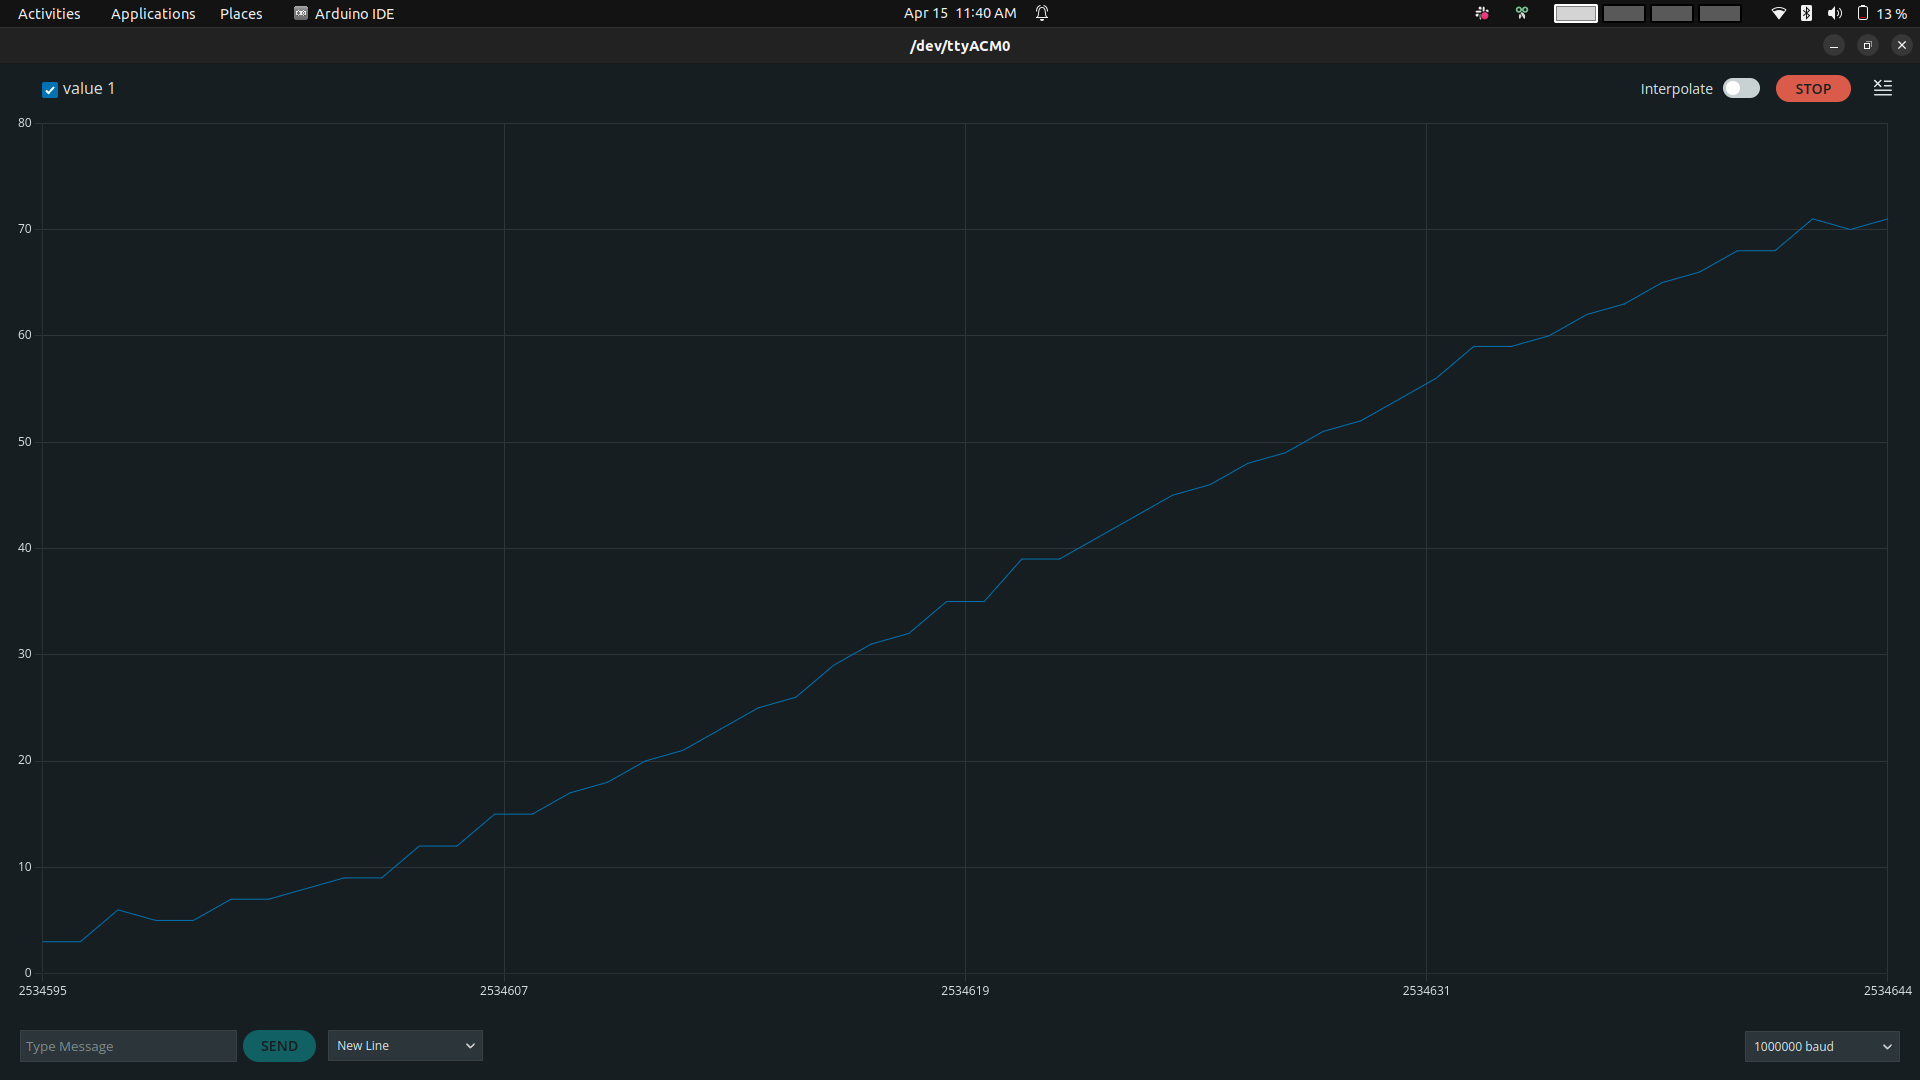
\includegraphics[scale=0.2]{figures/periodic_noise.png}
          \caption{60Hz signal}
        \end{figure}

        \begin{figure}[H]
          \centering
          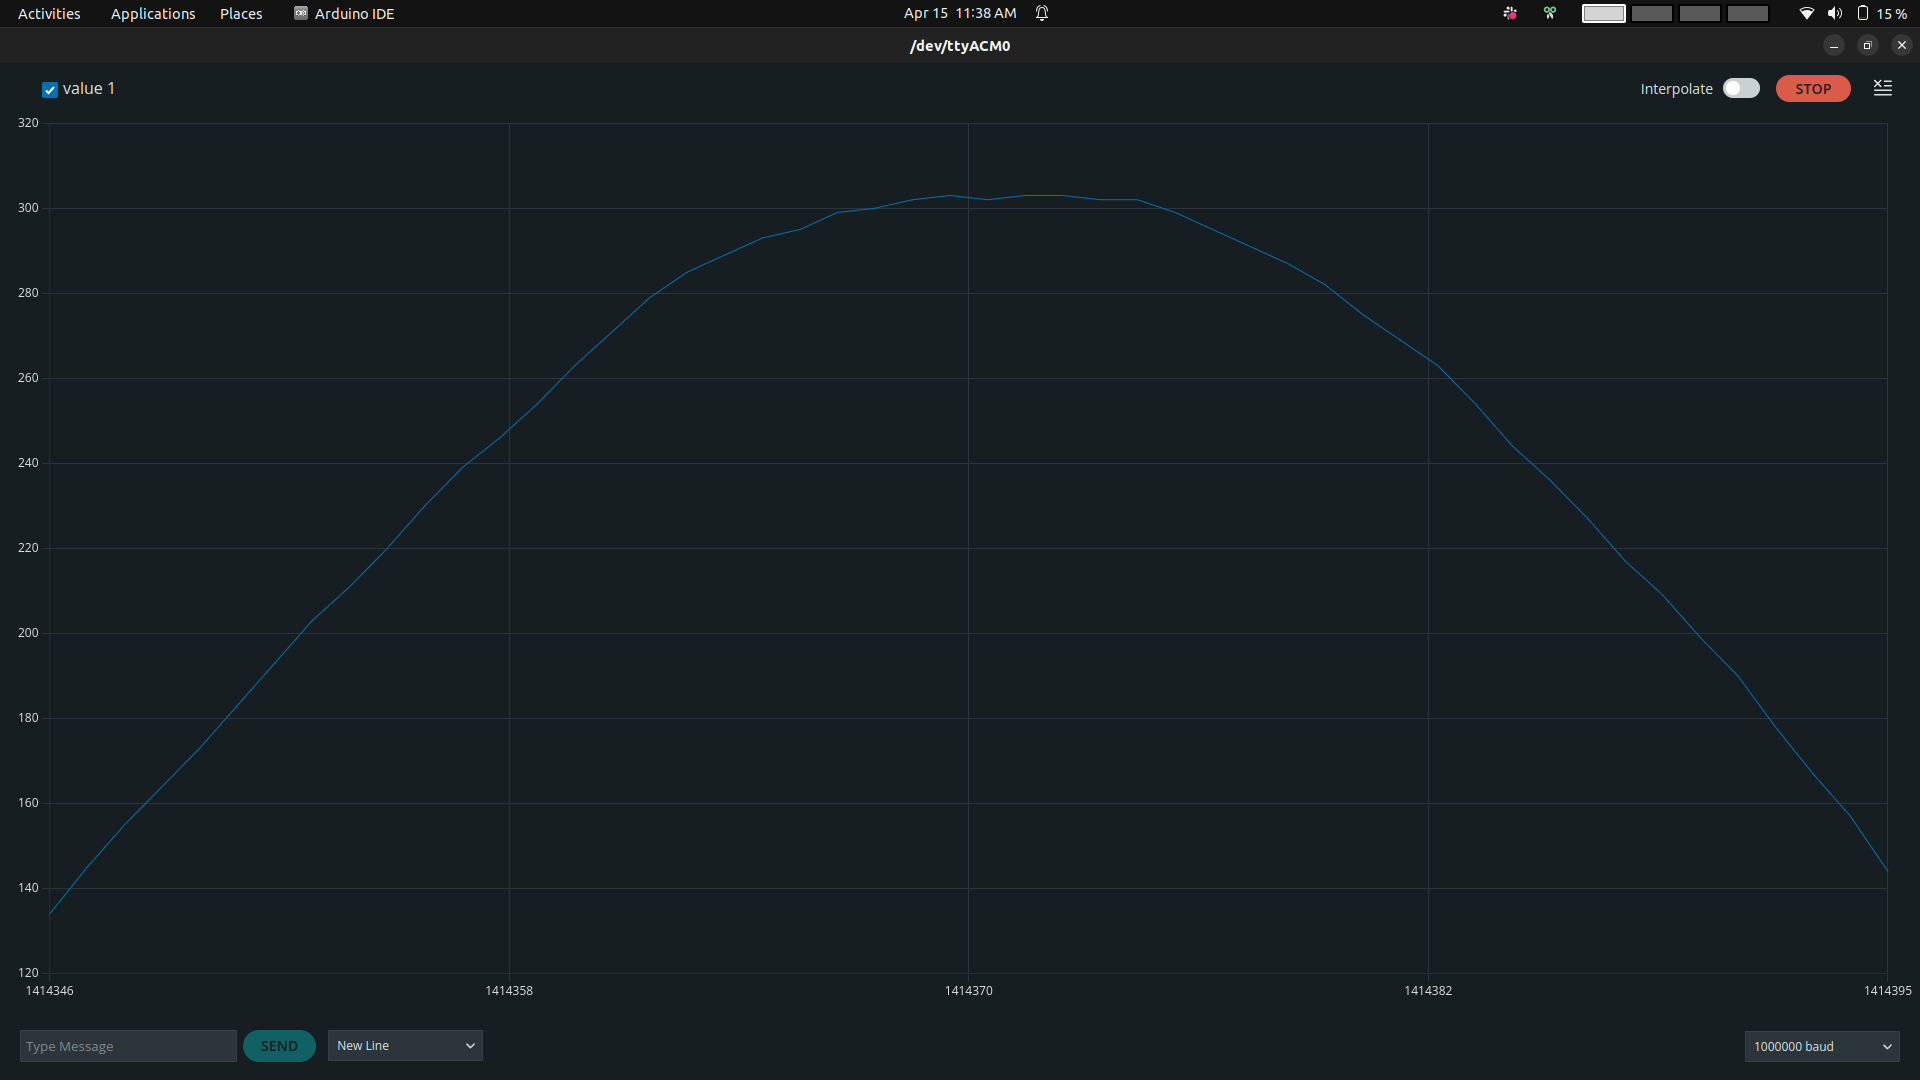
\includegraphics[scale=0.2]{figures/periodic_noise2.png}
          \caption{60Hz signal}
        \end{figure}

\end{itemize}
\subsection{Initial Readings with Averaging}
When I first started taking measurements with averaging
\begin{itemize}
  \item At the start, without enough readings to plot the data, I observed peaks in the readings. These peaks were caused by the insufficient data points for proper averaging.
  \item As I continued to take more readings over time, the peaks gradually diminished, and the readings became more stable. This stabilization was a result of the increasing number of data points being averaged.
  \item To further improve the stability of the readings, I introduced a slight delay by taking some dummy readings at the beginning. This delay allowed the averaging process to stabilize before I started plotting the actual data, resulting in fewer peaks and a more stable signal.
        \begin{figure}[H]
          \centering
          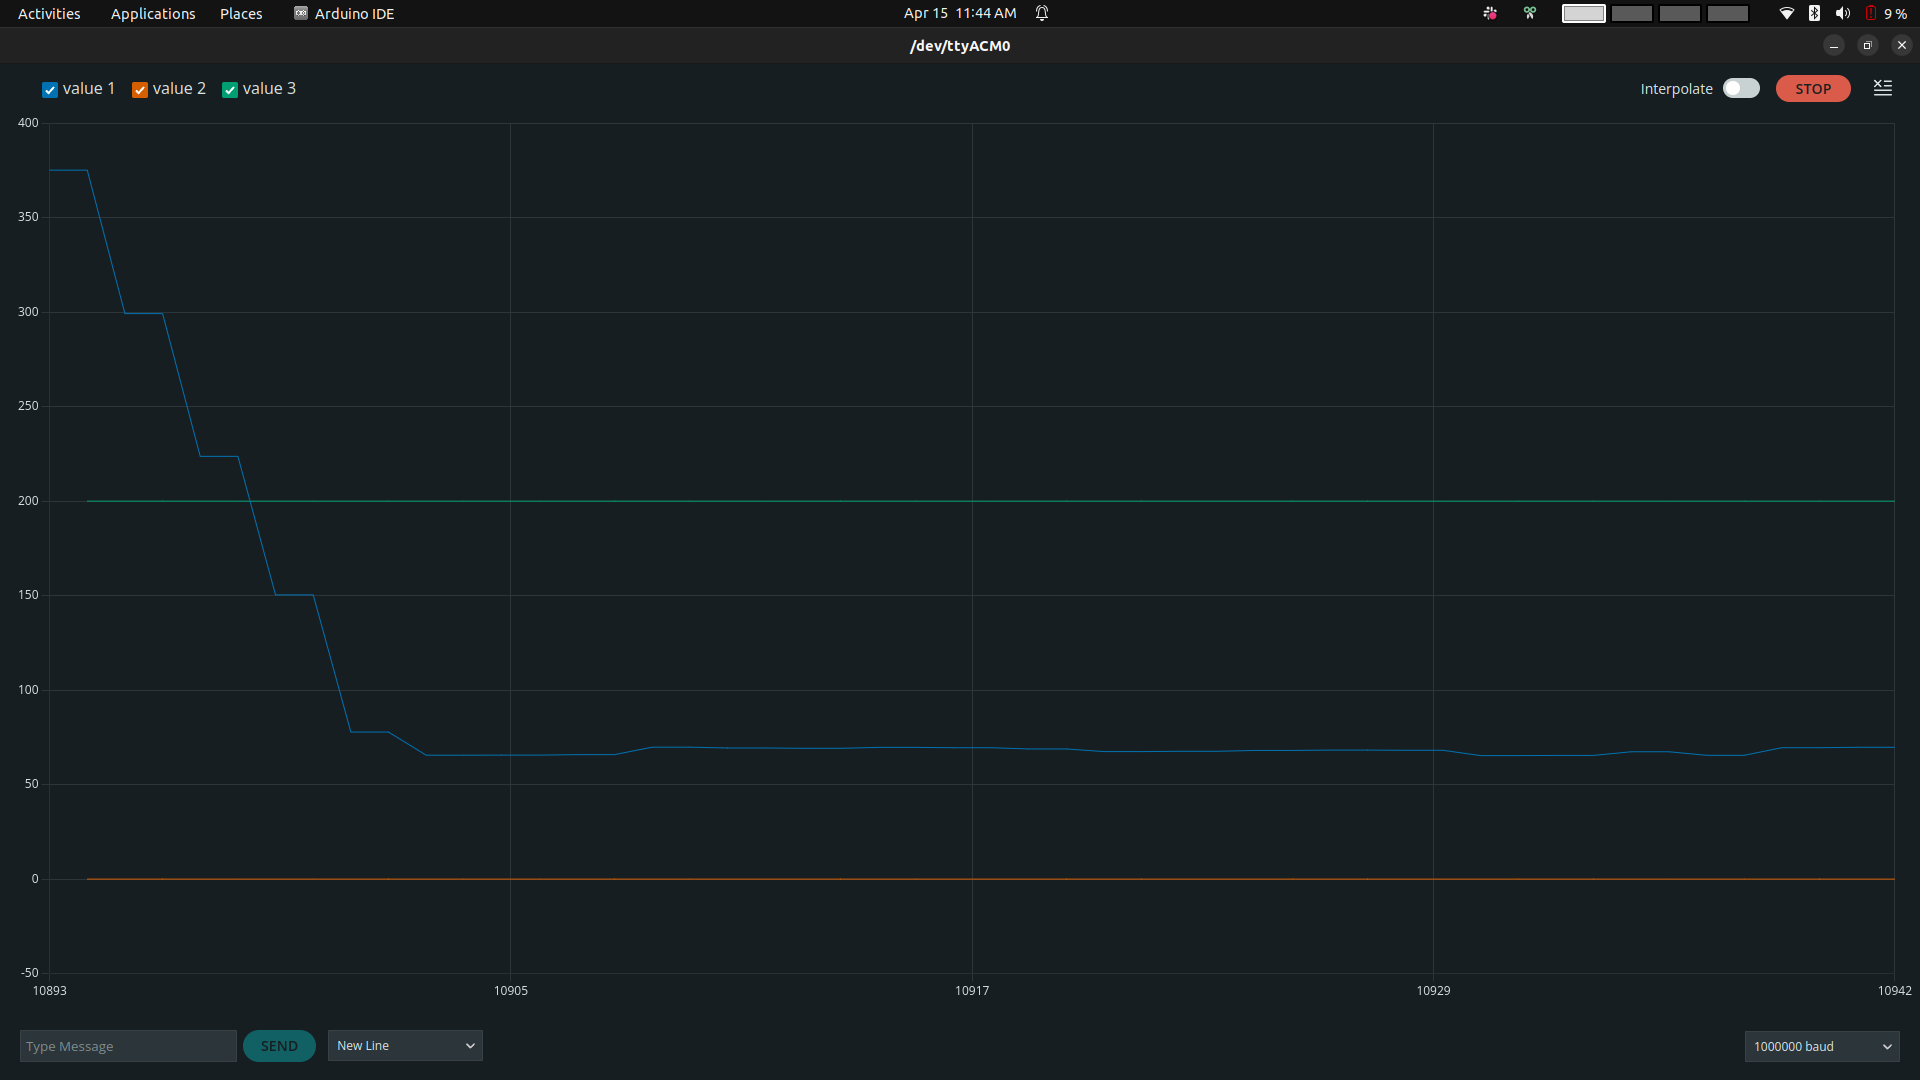
\includegraphics[scale=0.2]{figures/initial_peak.png}
          \caption{Without adding dummy readings at first}
        \end{figure}

        \begin{figure}[H]
          \centering
          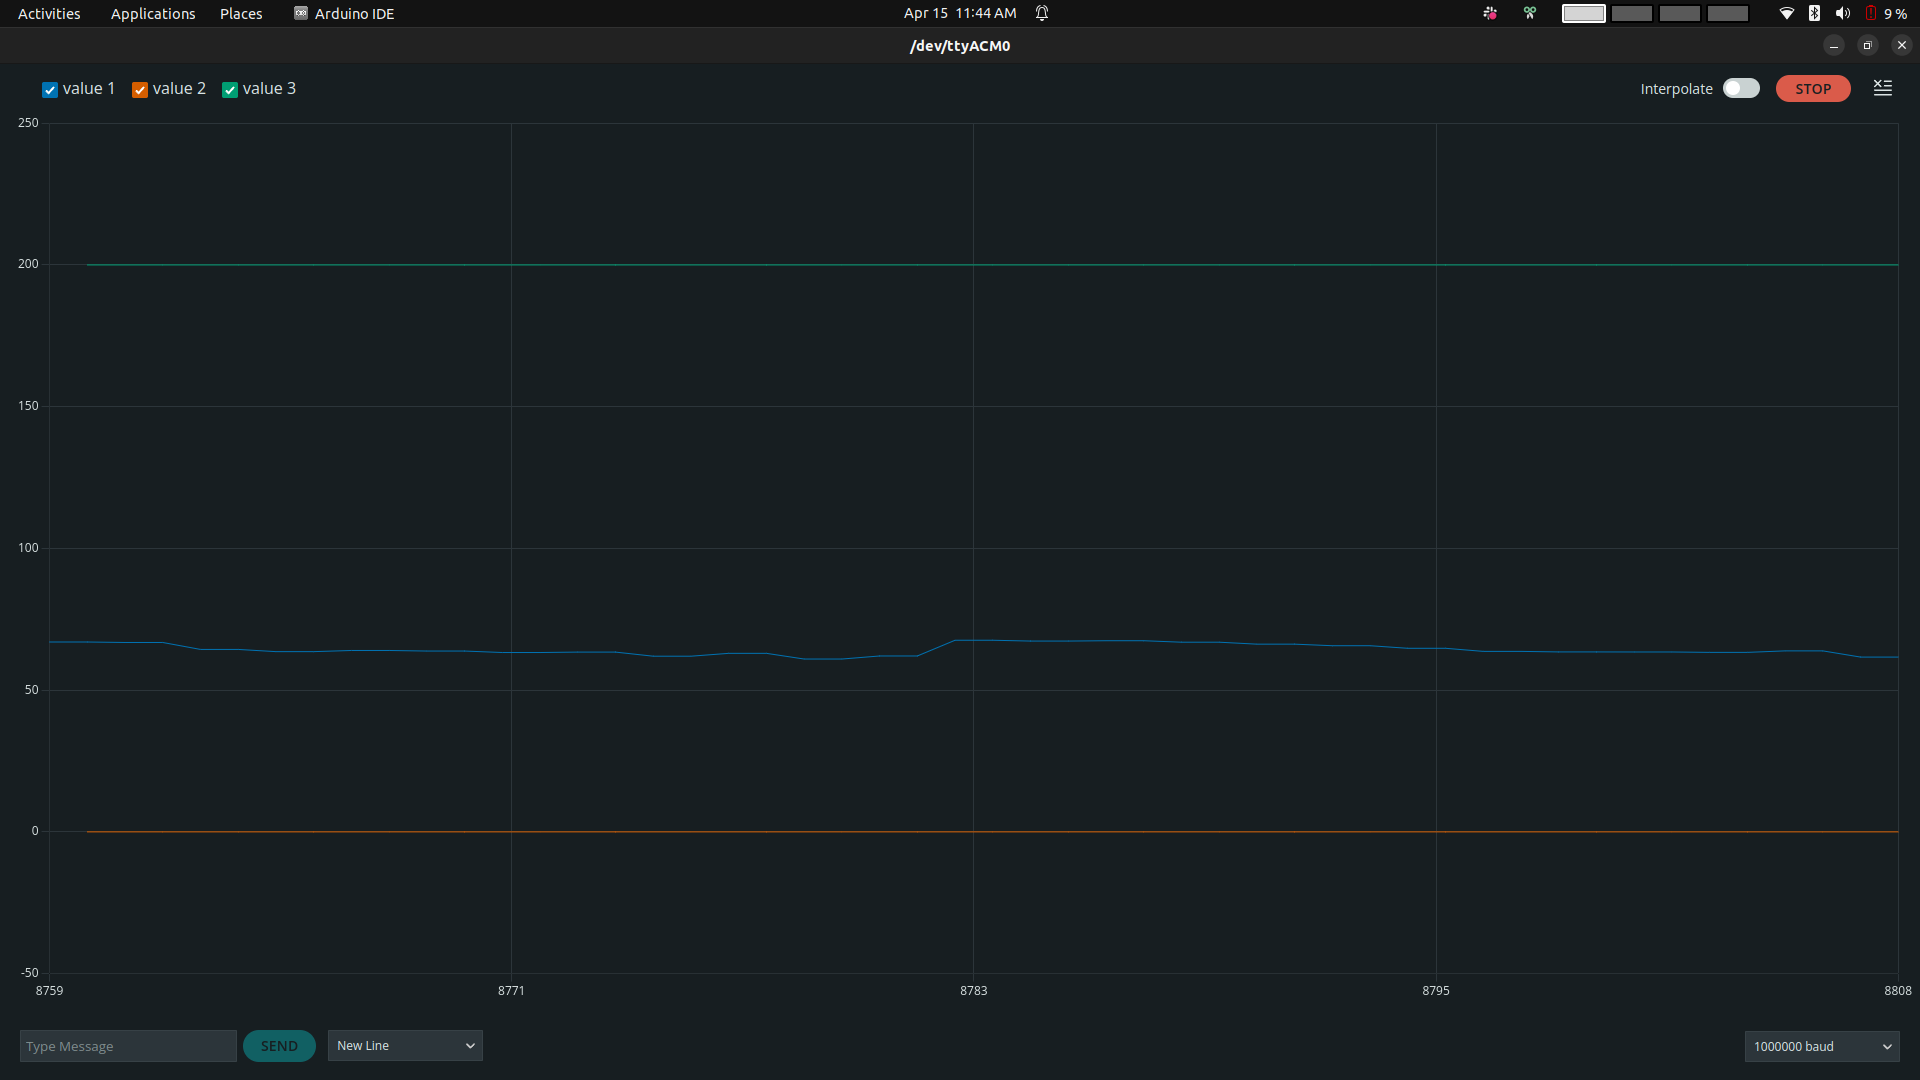
\includegraphics[scale=0.2]{figures/after_stabilizing.png}
          \caption{After Adding dummy readings in setup()}
        \end{figure}

        \begin{table}[H]
          \centering
          \begin{tabular}{|c|c|}
            \hline
            Initial peak without dummy Readings & Initial readings with dummy readings \\
            \hline
            400 ADU                             & 40 ADU                               \\
            \hline
          \end{tabular}
        \end{table}

\end{itemize}
\subsection{Triboelectric Charging}
Triboelectric charging occurs when two different materials are rubbed together, causing electrons to transfer from one material to the other. This transfer of electrons results in the accumulation of static charges on the surfaces of the materials. I investigated this phenomenon using various materials and observed the corresponding changes in the E-field meter readings.
\begin{itemize}
  \item Rubbing Scale against hair: When a scale was rubbed against the experimenter's hair and brought near the E-field meter antenna, the readings showed a strong negative polarity, with peaks reaching -1000 ADU. This indicates that the scale acquired a large negative charge through triboelectric charging.
        \begin{figure}[H]
          \centering
          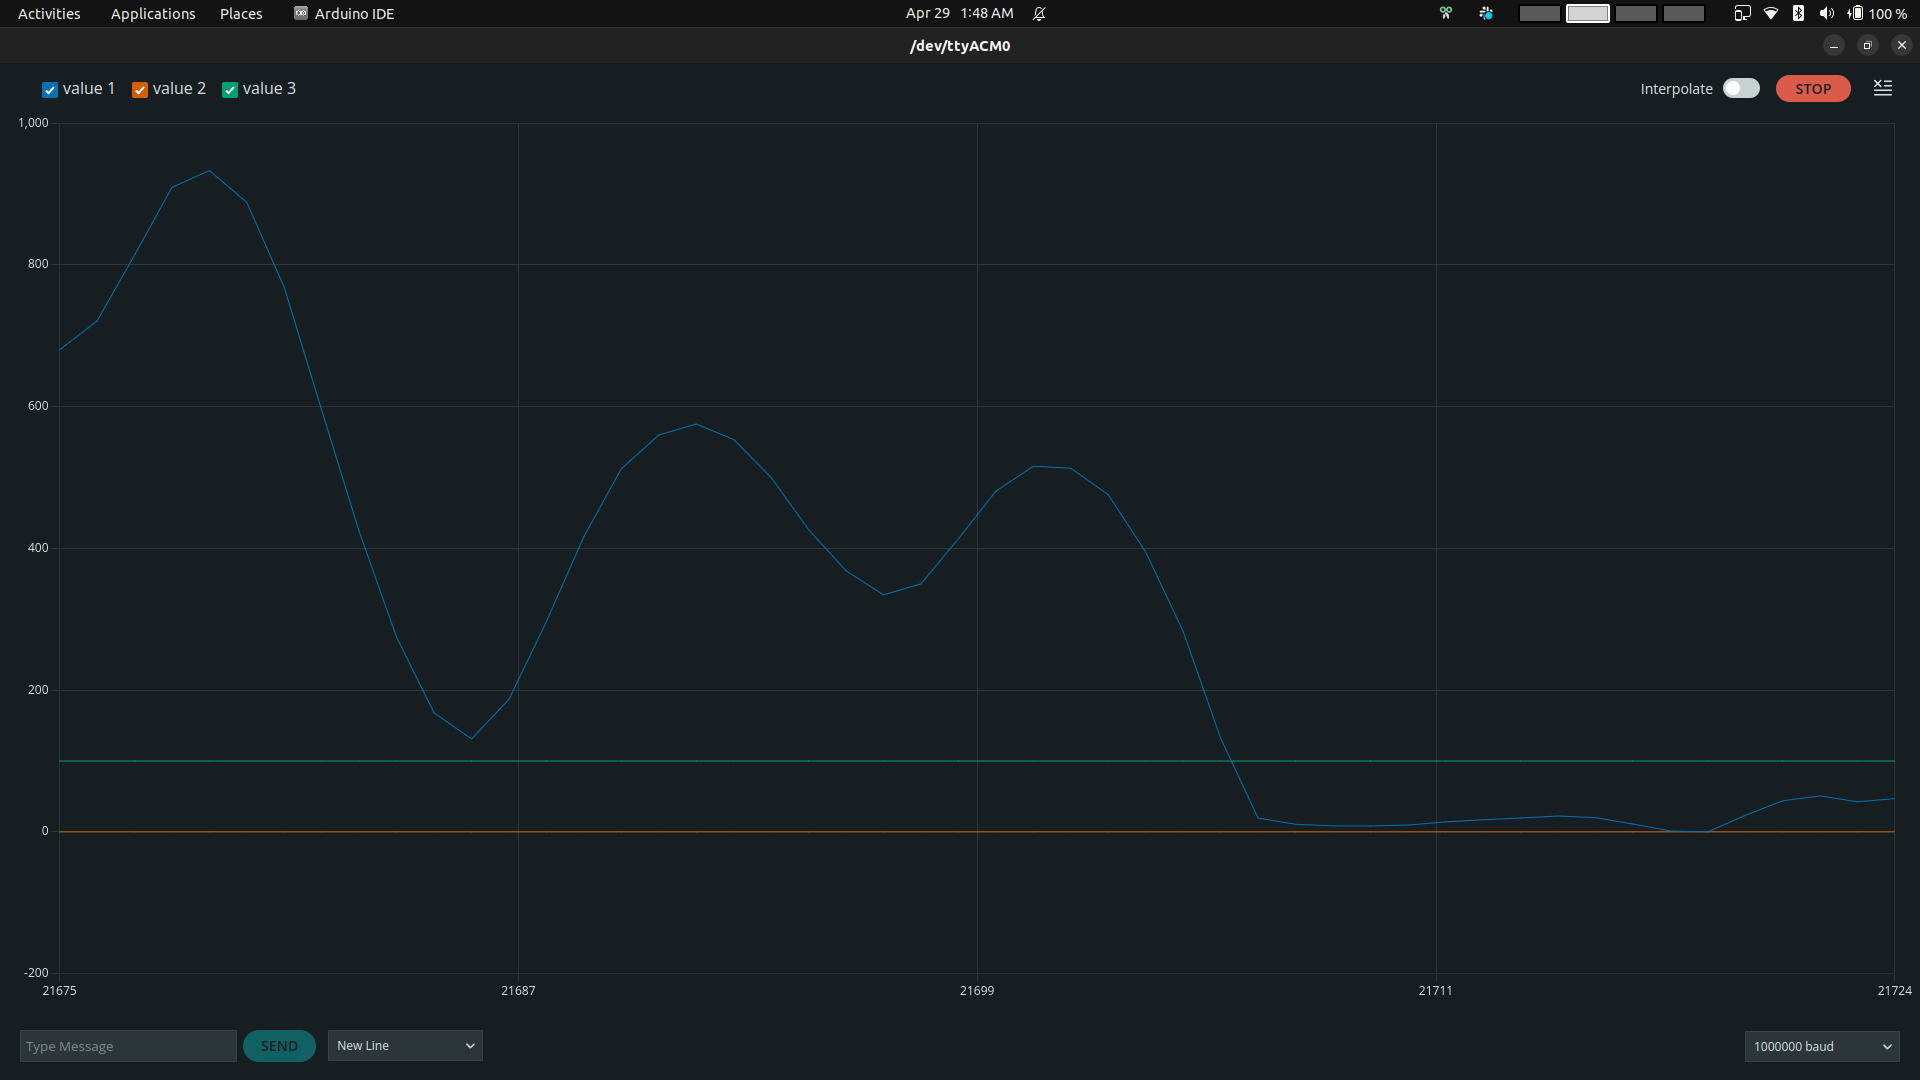
\includegraphics[scale=0.2]{figures/scale.png}
          \caption{Charged Scale}
        \end{figure}

  \item Rubbing hand against hair: When a hand was rubbed against the experimenter's hair and brought near the E-field meter antenna, the readings showed a strong negative polarity, with peaks reaching -200 ADU. This indicates that the hand acquired a negative charge through triboelectric charging.
        \begin{figure}[H]
          \centering
          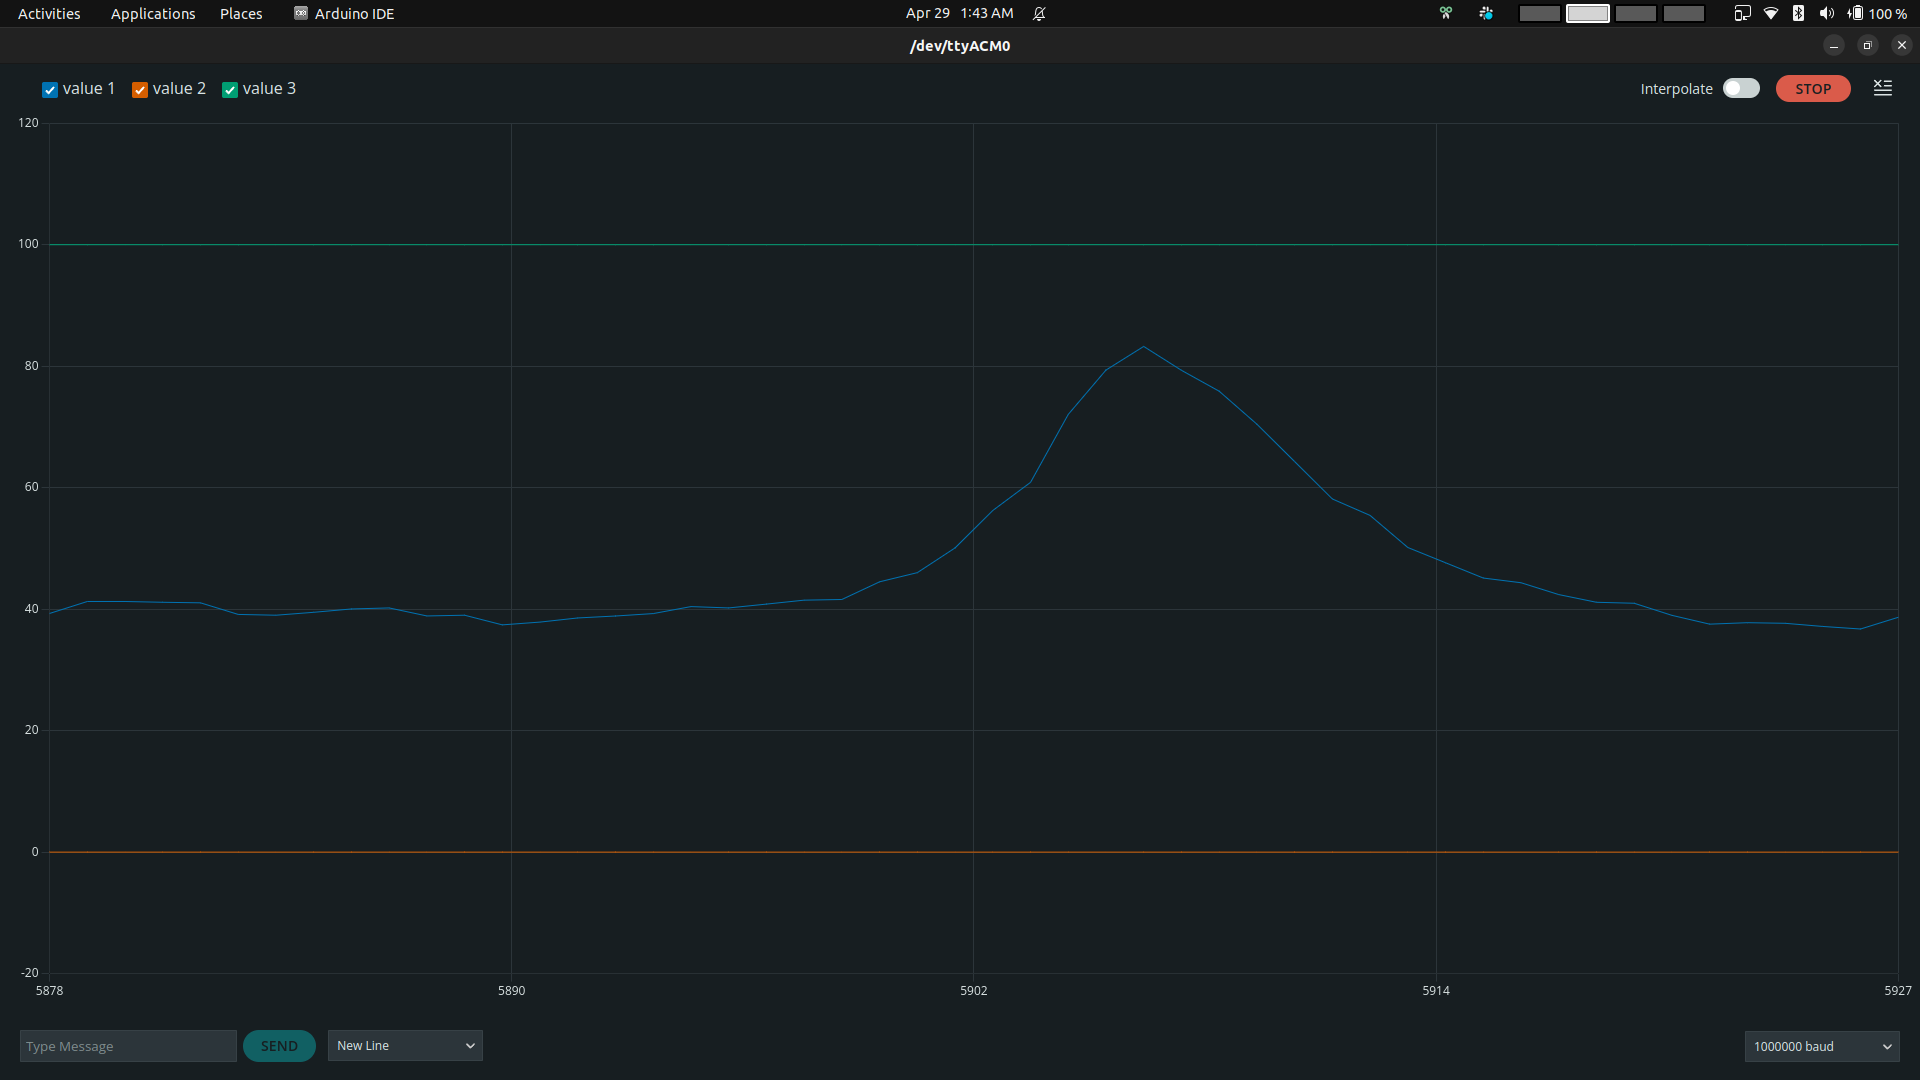
\includegraphics[scale=0.2]{figures/hand.png}
          \caption{Charged Hand}
        \end{figure}

        \begin{table}[H]
          \centering
          \begin{tabular}{|c|c|}
            \hline
            Charged Hand & Charged Scale \\
            \hline
            900 ADU      & 80 ADU        \\
            \hline
          \end{tabular}
        \end{table}

\end{itemize}
These experiments demonstrate how triboelectric charging can generate significant static charges on various materials, which can be detected and measured using the E-field meter.
\subsection{ESD Mitigation Techniques}
To minimize the risk of ESD damage to sensitive electronic components, it is essential to implement effective ESD mitigation techniques.
\begin{itemize}
  \item Grounding: When a charged object was touched to a grounded metal surface, the E-field meter readings quickly returned to the baseline level (-40 ADU). This rapid return to the baseline indicates that the static charges were effectively dissipated through grounding, neutralizing the object's charge.

        \begin{figure}[H]
          \centering
          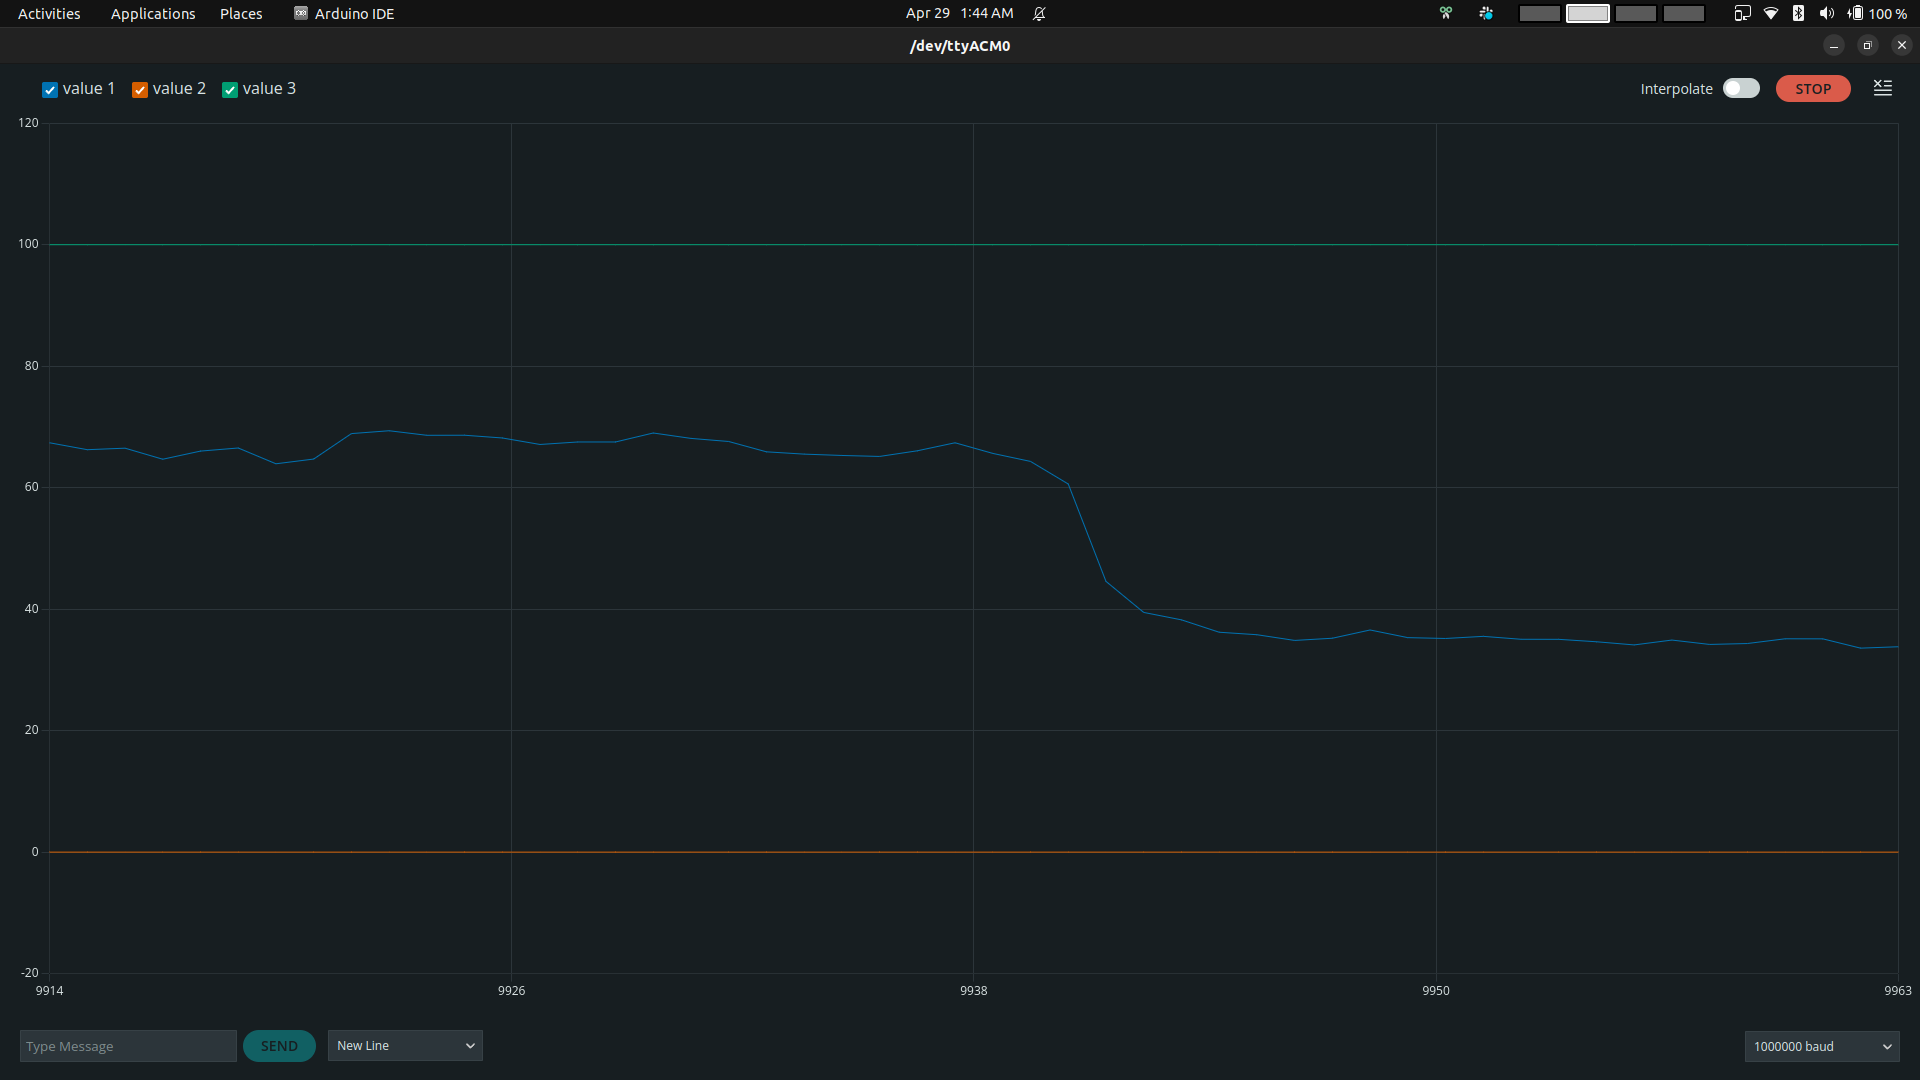
\includegraphics[scale=0.2]{figures/hand_when_touching_groung.png}
          \caption{The falling edge when I touch ground with hand close the antenna}
        \end{figure}

        \begin{table}[H]
          \centering
          \begin{tabular}{|c|c|}
            \hline
            Without Grounding & With Grounding \\
            \hline
            80 ADU            & 40 ADU         \\
            \hline
          \end{tabular}
        \end{table}



\end{itemize}
These observations highlight the importance of proper ESD mitigation techniques in preventing the buildup of harmful static charges that can damage sensitive electronics.
\subsection{Distance and Orientation Effects}
The distance and orientation of the charged object relative to the E-field meter antenna play a significant role in the magnitude of the readings.
\begin{itemize}
  \item Distance: As the charged object was brought closer to the antenna, the E-field meter readings increased in magnitude. Conversely, moving the object away from the antenna resulted in a decrease in the readings. This relationship between distance and field strength is consistent with the inverse square law, which states that the magnitude of an electric field decreases with the square of the distance from the charge.


        \begin{figure}[H]
          \centering
          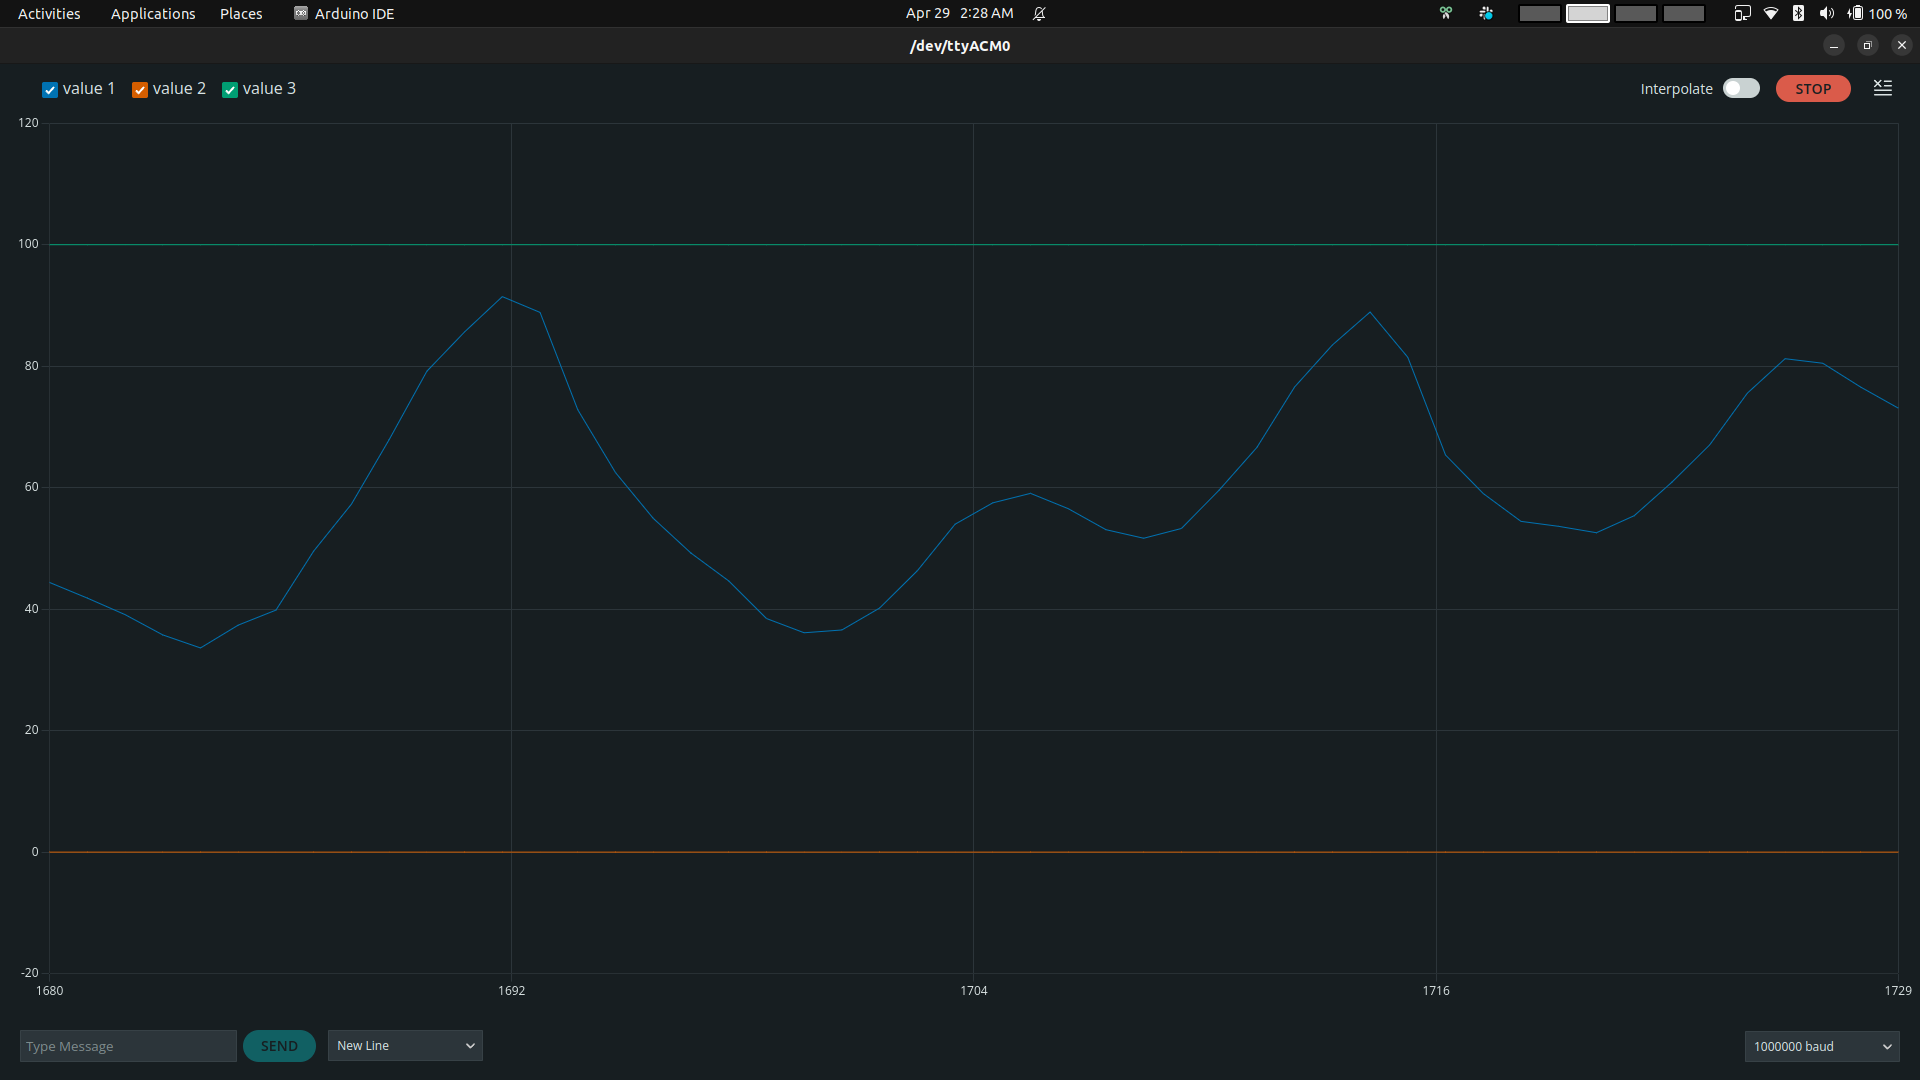
\includegraphics[scale=0.2]{figures/large_distance.png}
          \caption{Large Distance between scale and antenna(about 10cm)}
        \end{figure}

        \begin{figure}[H]
          \centering
          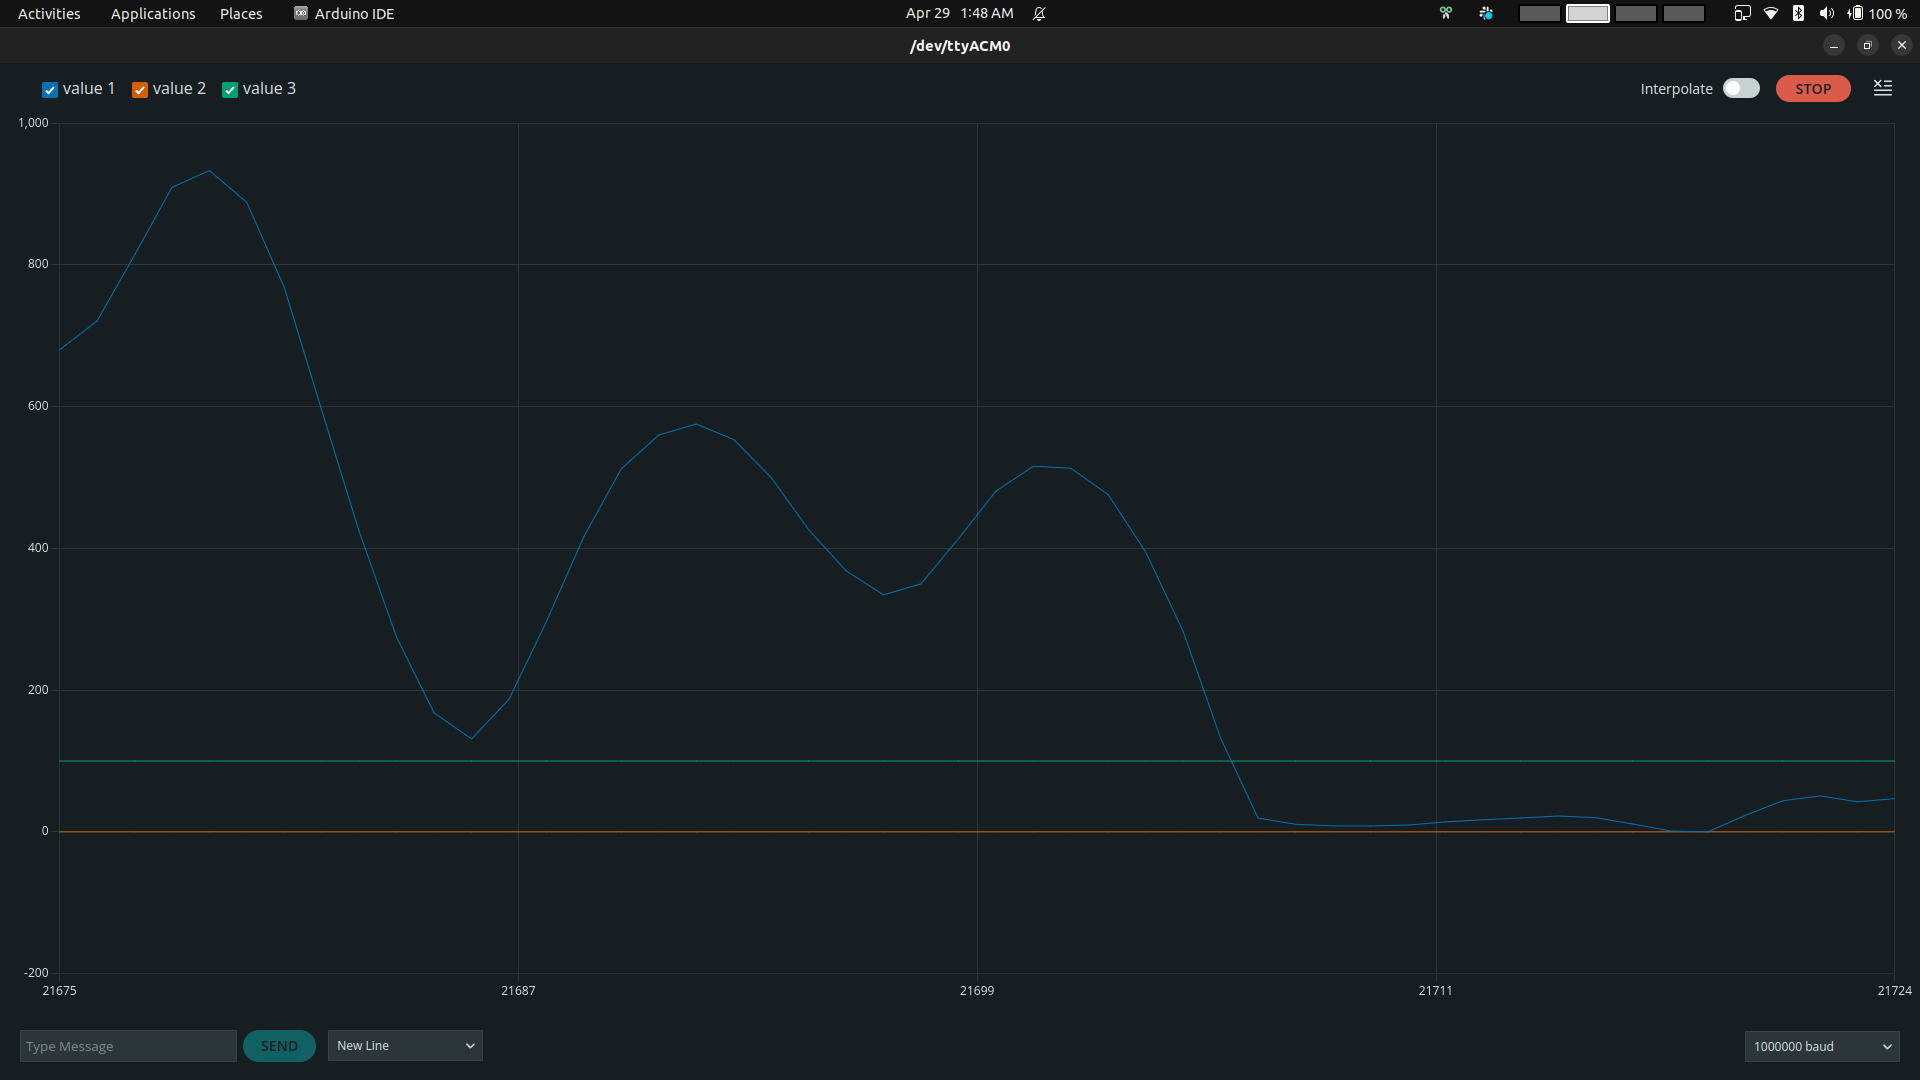
\includegraphics[scale=0.2]{figures/scale.png}
          \caption{Small Distance between scale and antenna(about 2cm)}
        \end{figure}

        \begin{table}[H]
          \centering
          \begin{tabular}{|c|c|}
            \hline
            Distance & ESD Voltage \\
            \hline
            10cm     & 90 ADU      \\
            2cm      & 900 ADU     \\

            \hline
          \end{tabular}
        \end{table}


  \item Orientation: The orientation of the charged object relative to the antenna also influenced the readings. When the charged surface was parallel to the antenna, the highest readings were observed. In contrast, when the charged surface was perpendicular to the antenna, lower readings were recorded. This difference in readings can be attributed to the direction of the electric field lines emanating from the charged surface.



        \begin{figure}[H]
          \centering
          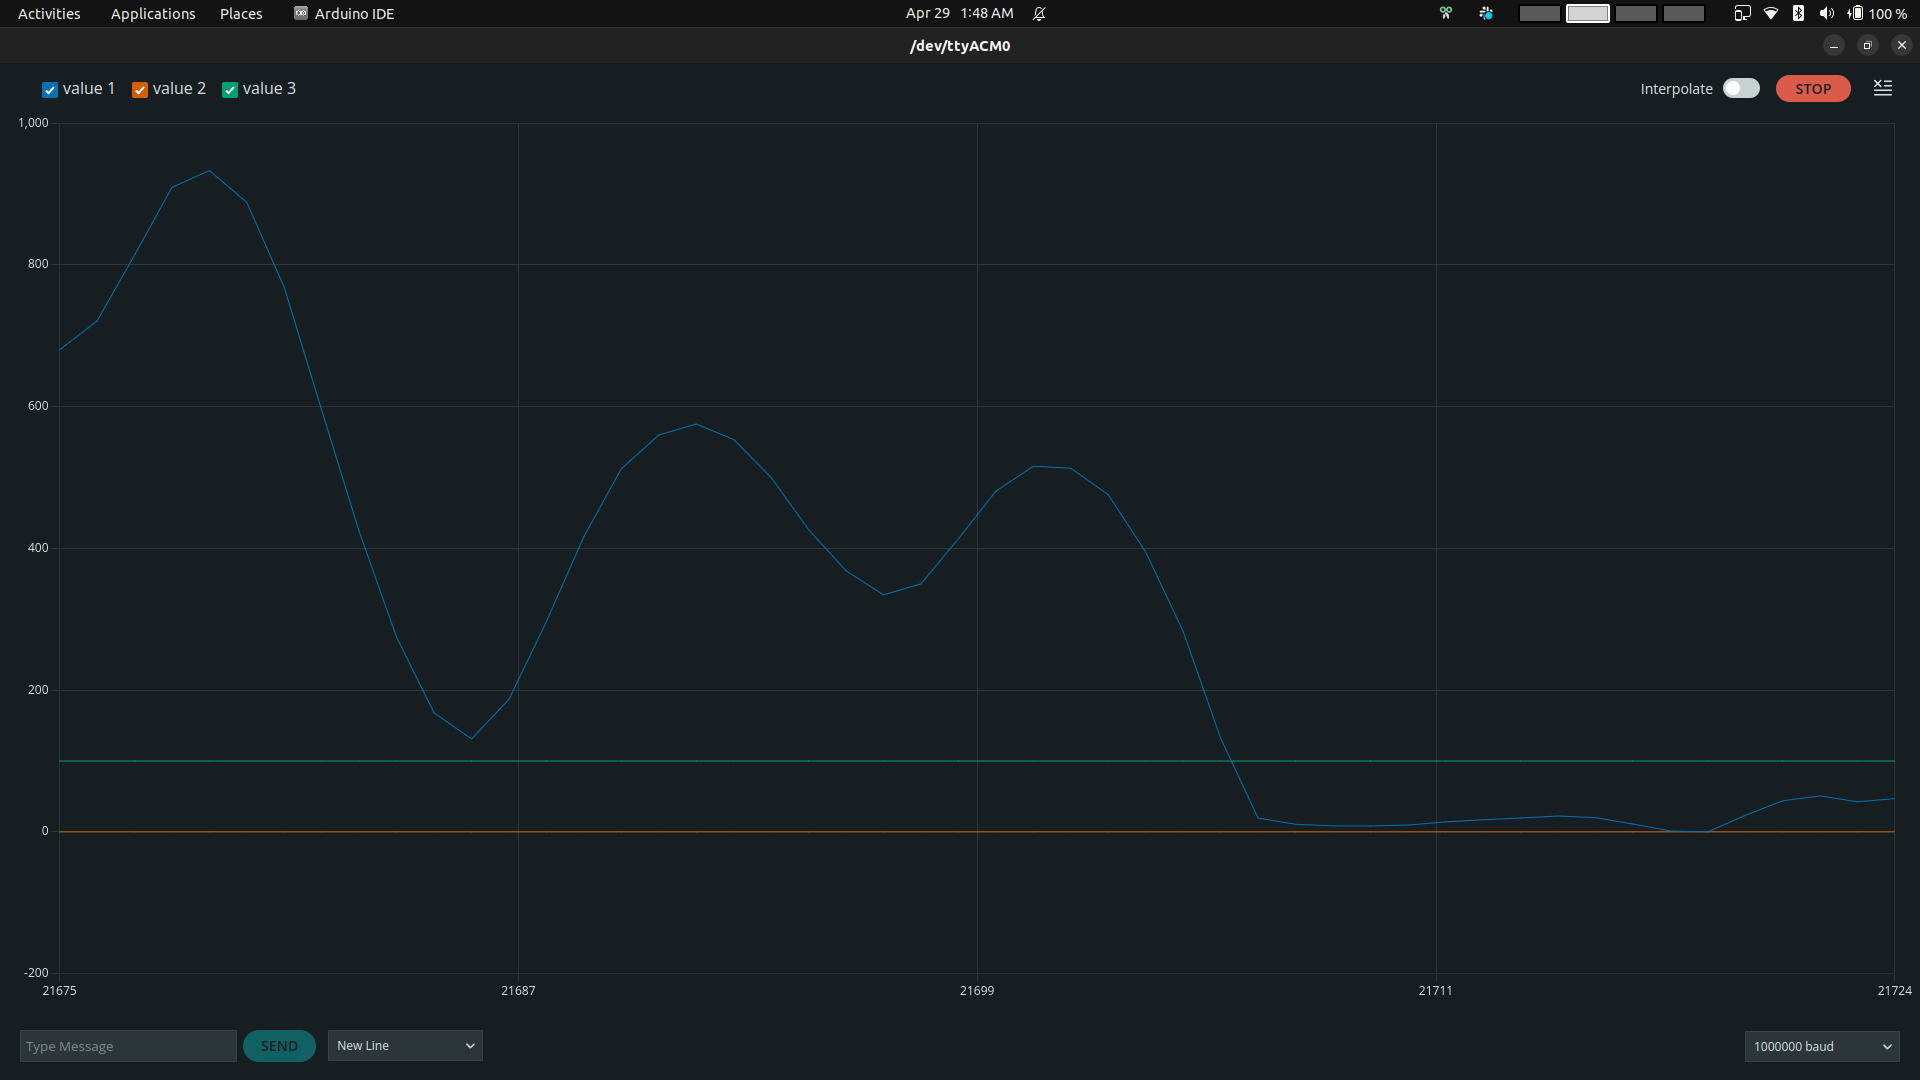
\includegraphics[scale=0.2]{figures/scale.png}
          \caption{Scale parallel to antenna}
        \end{figure}

        \begin{figure}[H]
          \centering
          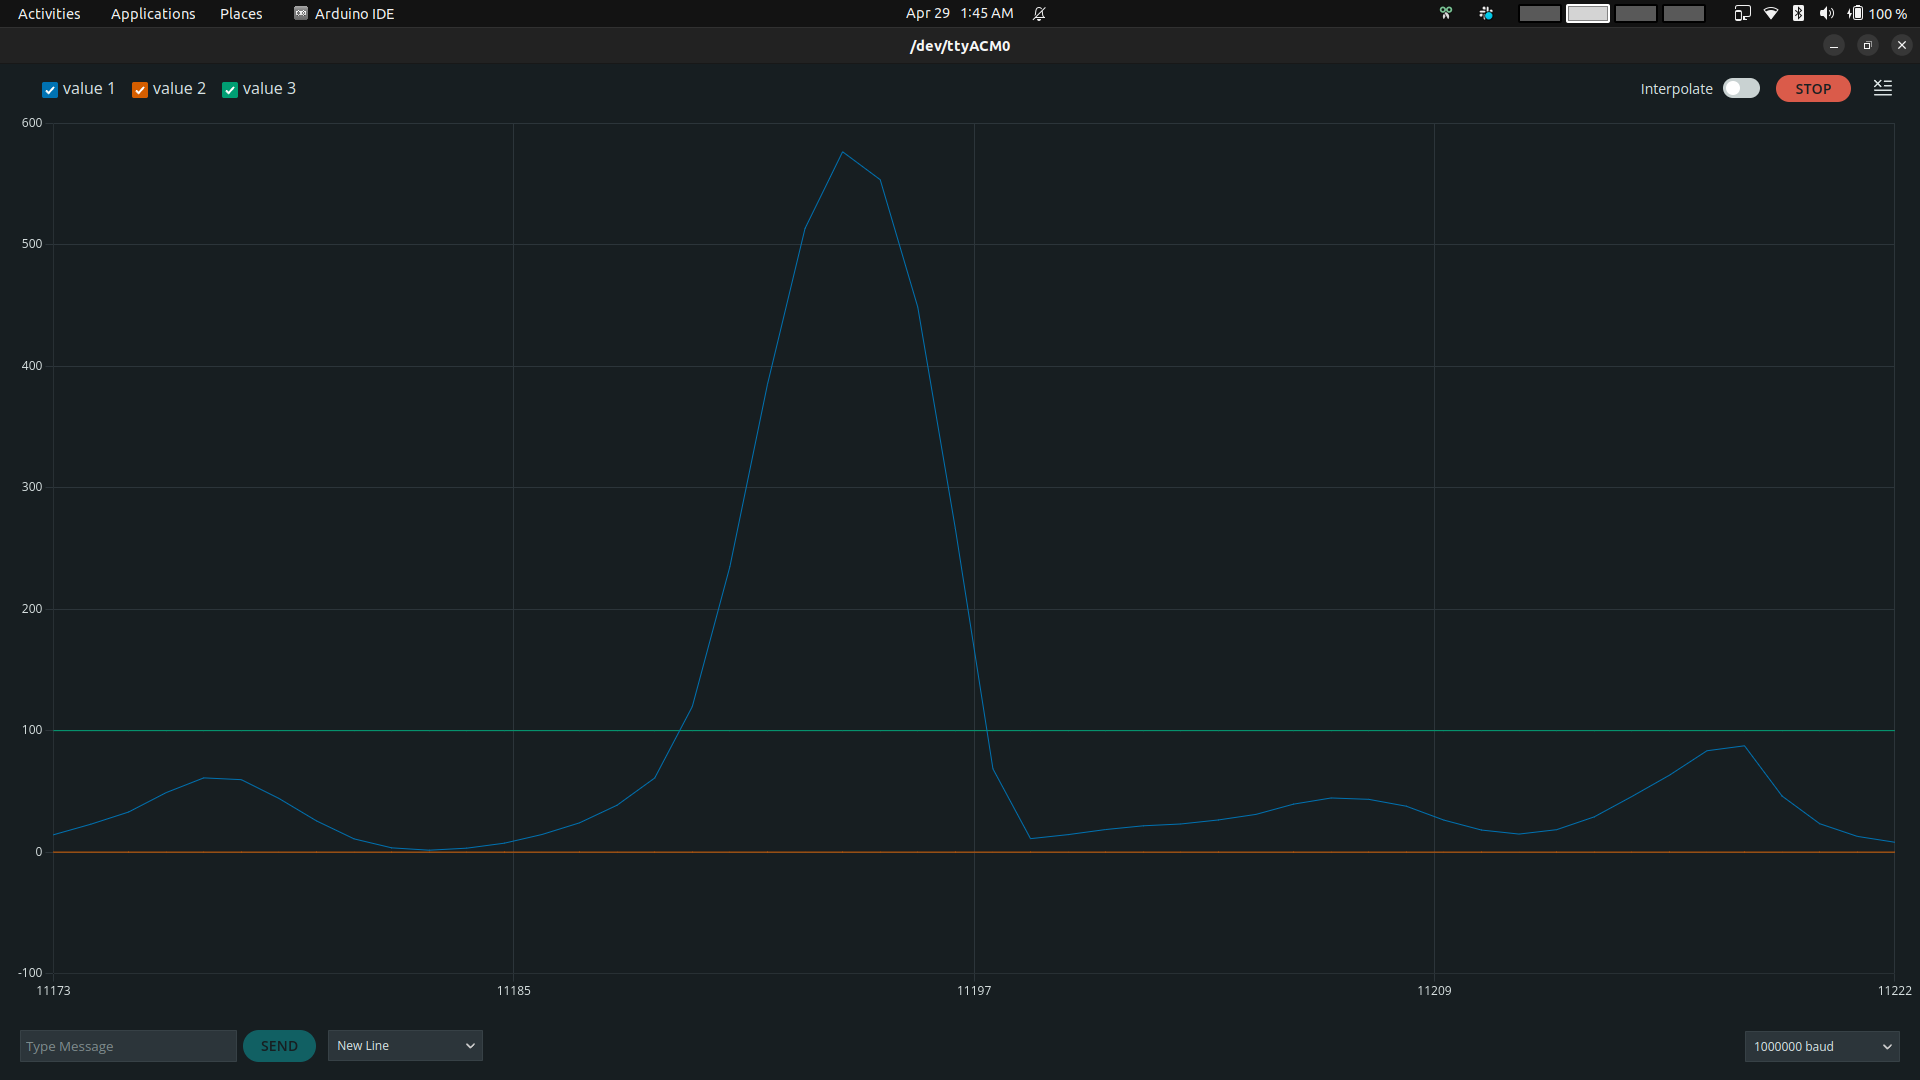
\includegraphics[scale=0.2]{figures/scale_perpenndicular.png}
          \caption{Scale perpendicular to antenna}
        \end{figure}


        \begin{table}[H]
          \centering
          \begin{tabular}{|c|c|}
            \hline
            Orientation              & ESD charge \\
            \hline
            Perpendicular to antenna & 550 ADU    \\
            Parallel                 & 900 ADU    \\

            \hline
          \end{tabular}
        \end{table}


\end{itemize}
Understanding the effects of distance and orientation on the E-field meter readings is crucial for accurately interpreting the results and optimizing the placement of the antenna in ESD-sensitive environments.


\section{Learnings and Observation}
% \begin{enumerate}
%   \item Practical circuit design and implementation: The lab provided hands-on experience in designing and constructing a custom instrument (Instrument Droid) for characterizing voltage sources and regulators. This involved selecting appropriate components, considering power dissipation, and implementing measurement techniques, reinforcing the importance of careful design and analysis.
%   \item Integration of multiple subsystems: The Instrument Droid involved the integration of various subsystems, including a microcontroller, DAC, ADC, op-amp, and MOSFET. Coordinating the operations of these subsystems and ensuring proper interfacing and communication was a valuable learning experience in system integration and design.
%   \item Noise management and signal conditioning: The lab highlighted the impact of noise and signal integrity on measurements. Techniques such as differential voltage measurement and proper grounding practices were essential for obtaining accurate and reliable results, reinforcing the importance of noise management and signal conditioning in electronic circuit design.
%   \item Data analysis and visualization: The lab involved collecting and processing measurement data, calculating parameters, and plotting the results. This reinforced the importance of data analysis, visualization, and interpretation in characterizing and understanding the behavior of electronic systems.
% \end{enumerate}\

\begin{enumerate}
  \item  Digital filtering techniques, such as power line cycle averaging, can effectively eliminate background noise and improve the meter's sensitivity.

  \item Understanding the concept of triboelectric charge separation is crucial for recognizing the sources of static charge buildup.
  \item The E-field meter's functionality relies on the Arduino's ADC and the antenna's ability to detect static electric fields.

  \item Averaging ADC readings over a specific time period helps to reduce noise and improve signal stability.
  \item Constructing an Arduino-based E-field meter enables the exploration of ESD principles and mitigation techniques.
  \item Digital filtering techniques, such as power line cycle averaging, can effectively eliminate background noise and improve the meter's sensitivity.

  \item Understanding the concept of triboelectric charge separation is crucial for recognizing the sources of static charge buildup.
        The E-field meter's functionality relies on the Arduino's ADC and the antenna's ability to detect static electric fields.

  \item Recognizing the effectiveness of ESD mitigation techniques, such as grounding and the use of ESD-safe materials, is crucial for maintaining a static-safe environment.

\end{enumerate}





\section{Conclusion}
\begin{enumerate}
  \item The Arduino ESD E-field Meter Lab provides a comprehensive hands-on experience in exploring the principles of electrostatic discharge and its mitigation techniques. By constructing an E-field meter using an Arduino and implementing digital filtering techniques, participants gain a deeper understanding of how static electric fields can be detected and measured.
  \item The lab demonstrates the significance of triboelectric charge separation in generating static charges and highlights the importance of implementing effective ESD mitigation strategies, such as grounding and the use of ESD-safe materials. The measurements obtained during the lab showcase the meter's sensitivity to static electric fields and illustrate the influence of factors such as distance, orientation, and charge dissipation on the magnitude of the readings.
  \item the lab emphasizes the value of hands-on experimentation in solidifying theoretical concepts and provides participants with practical experience in using the Arduino platform for sensor interfacing and data processing. The code examples and measurement results serve as references for future projects involving ESD detection and mitigation.
\end{enumerate}

% \begin{enumerate}
%   \item The Instrument Droid proved to be an effective tool for characterizing voltage sources and regulators by measuring their Thevenin parameters. By sweeping the load current and measuring the corresponding output voltages, the Instrument Droid could accurately determine the Thevenin voltage and Thevenin resistance.
%   \item Verification with known sources, such as a function generator and a bench power supply with a known series resistor, confirmed the accurate operation of the Instrument Droid. This approach allowed for the identification and resolution of any potential issues before proceeding to characterize unknown sources.
%   \item The Instrument Droid successfully characterized various unknown voltage sources, including wall warts, batteries, Arduino outputs, op-amp outputs, and other voltage sources commonly found in electronics laboratories. The measured Thevenin parameters and resistance curves provided valuable insights into the behavior and characteristics of these sources under varying load conditions.
%   \item Comparing the measured Thevenin parameters and resistance curves with theoretical expectations or manufacturer specifications for well-understood voltage sources, such as batteries and regulated power supplies, allowed for further investigation and discussion, deepening the understanding of the underlying principles and potential sources of error.
%   \item The pulsed current measurement approach implemented in the Instrument Droid effectively managed power dissipation, preventing overheating and potential damage to circuit components, especially when characterizing high-current voltage sources.
%   \item The lab experience reinforced the importance of a systematic approach, attention to detail, and the ability to analyze and interpret data in the context of theoretical principles and practical considerations when designing and testing electronic circuits and instrumentation systems.
% \end{enumerate}







\vspace{50px}
\hrule
\hrule

\pagebreak





%---------------------------------------------------------------------------
\end{document}

